\chapter{Experimental Results}
\label{chap:result}

Defined at the end of the Chapter~\ref{chap:intro}, the four objectives of this thesis are to augment the COACH system with an emotional reasoning engine based on BayesACT so that the augmented system: (1) is designed in a portable and extensible way; (2) runs in real-time from the perspective of the user group; (3) provides at least a level of functional assistance of as high quality as the COACH; (4) is able to tune the prompts in some way according to the emotional state of a user. It has been showed in the Chapter~\ref{chap:design} and Chapter~\ref{chap:impl} that the system we developed is easy to be extended. Experiments conducted on the system show that an average latency of 46.79ms is caused by the Observer component of the system, 0.009ms by the Buffer, and 1.65s by the Updater. The overall average latency of the system is around 1.70s, which means that the system runs in real-time from the perspective of its user group. 

We demonstrate in this section by laboratory based tests that the system is also able to provide a level of functional assistance and to produce system prompts that have encoded to some extent the emotional state of the user. The tests were conducted on a PC running 64-bit Ubuntu 12.04 LTS, with AMD FX(tm)-6300 Six-Core Processor × 6 and NVIDIA GeForce GTX 650 Ti Graphics Card. A kinect camera was mounted above the sink area and was the only sensor of the system.

\section{Parameter Setup}
This paragraph explains how the values of threshold variables $distance$ and $difference$ used in the EPA-Calculator were assigned based on statistical results obtained from experiments as follows. Videos were recorded while a person washed her hands with different emotions in nine complete hand-washing trials. A total number of 13703 frames were extracted from the videos. For each frame, the distances between the person's two hands were computed. For each pair of neighbouring frames, the distances that the person's hands moved between the frames were calculated as well. Histograms of the two ``distances'' are shown in figure 4-6 \textcolor{red}{TODO: modify this}. Note that in around 69\% of the frames, the distances between the user's hands falls into the range of $(8, 40]$. Note also that in around 70\% of frames, the distances the user's hands have moved from their positions in the last frames falls into the range of $(3.5, 17.5]$. Based on analysis of the the distributions of the two ``distances'', we assigned the values of variables used in the EPA-Calculator as following: $distance = \{-\infty, 0, 8, 40, 128, 160, +\infty\}$, $potency = \{-4.3, -4.3, 0, 1, 2, 4.3, 4.3\}$, $difference = \{-\infty, 0, 3.5, 17.5, 35, 70, +\infty\}$, and $activity = \{-4.3, -4.3, -2, -1, 0, 4.3, 4.3\}$. Table~\ref{table:param-setting} shows an overview of the values assigned to important variables in our tests of the system. 

%
% TODO: insert figure 4-6 here

%
% table: Parameter values used in laboratory experiments
\begin{table}
\centering
\caption{Parameter values used in laboratory experiments}
\label{table:param-setting}
\begin{tabular}{| l | l | l |}
\hline
\textbf{Param.} & \textbf{Value} & \textbf{Defined in which component} \\ \hline
$n$ & $10$ & EPA-Calc \\ \hline
$distance$ & $\{-\infty, 0, 8, 40, 128, 160, +\infty\}$ & EPA-Calc \\ \hline
$potency$ & $\{-4.3, -4.3, 0, 1, 2, 4.3, 4.3\}$ & EPA-Calc \\ \hline 
$difference$ & $\{-\infty, 0, 3.5, 17.5, 35, 70, +\infty\}$ & EPA-Calc \\ \hline
$activity$ & $\{-4.3, -4.3, -2, -1, 0, 4.3, 4.3\}$ & EPA-Calc \\ \hline
$alpha$ & $0$ & Buffer \\ \hline
$timeout$ & $300$ & Buffer \\ \hline
$timeup$ & $1$ & Buffer \\ \hline
$\beta_{a}^{0}$ & $0.001$ & Updater \\ \hline
$\beta_{c}^{0}$ & $2.0$ & Updater \\ \hline
$\gamma$ & $(100000, 1.0, 0.5)$ & Updater \\ \hline
$N$ & $2000$ & Updater \\ \hline
$f\_a^{0}$ & $[1.5, 0.51, 0.45]$ & Updater \\ \hline
$f\_c^{0}$ & Different in each test &Updater \\ \hline
\end{tabular}
\end{table}

\section{Overview of Two Laboratory Tests}

%
% Table: results of test #1

\begin{center}
\begin{longtable}{| V{0.8cm} | V{2.6cm} | V{1.7cm} | V{2.1cm} | V{1.45cm} | V{1.6cm} | V{3.2cm} |}
\caption{State changes in test \#1 of the system}
\label{table:result-1}



\hline \multicolumn{1}{|c|}{\textbf{Time (s)}} & \multicolumn{1}{c|}{\textbf{Triple chosen}} & \multicolumn{1}{c|}{\textbf{Other feasible triples}} \\ \hline 
\endfirsthead

\multicolumn{3}{c}%
{{\bfseries \tablename\ \thetable{} -- continued from previous page}} \\
\hline \multicolumn{1}{|c|}{\textbf{Time (s)}} &
\multicolumn{1}{c|}{\textbf{Triple chosen}} &
\multicolumn{1}{c|}{\textbf{Other feasible triples}} \\ \hline 
\endhead

\hline \multicolumn{3}{|r|}{{Continued on next page}} \\ \hline
\endfoot

\hline \hline
\endlastfoot


Time &
User Behav. (screenshot) &
Behav. prop./epa &
Planstep Belief &
$f\_c$ &
Prompt: prop./epa &
Avatar (screenshot) \\ \hline


%column-1
t1 &
%column-2
\vskip 0.15cm
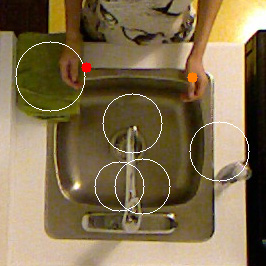
\includegraphics[width=\linewidth]{fig/system/_fast2-towel1_.jpg} &
%column-3
TOWEL
\vskip 0.2cm
$\begin{bmatrix}
0 \\
1.86 \\
-1.7
\end{bmatrix}$ &
%column-4
\begin{minipage}[c]{\linewidth} \centering
[1.00, 0.00, 0.00, 0.00, 0.00, 0.00, 0.00, 0.00] most likely planstep=0
\end{minipage} &
%column-5
$\begin{bmatrix}
1.7 \\
1.41 \\
-1.39
\end{bmatrix}$ &
%column-6
``turn on water''
\vskip 0.2cm
$\begin{bmatrix}
1.82 \\
0.22 \\
0.47
\end{bmatrix}$ &
%column-7
\vskip 0.15cm
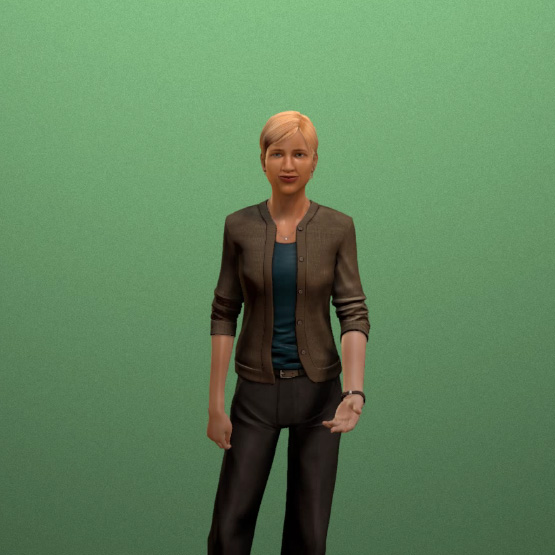
\includegraphics[width=2.6cm]{fig/prompt/_please-turn-on-the-water_.jpg}
\footnotesize
``Hello I am so glad to have you here. Please turn on the water.''
\\ \hline


%column-1
t2 &
%column-2
\vskip 0.15cm
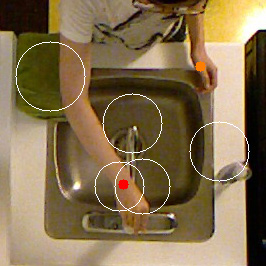
\includegraphics[width=\linewidth]{fig/system/_fast2-tap1_.jpg} &
%column-3
TAP
\vskip 0.2cm
$\begin{bmatrix}
0 \\
1.68 \\
-0.58
\end{bmatrix}$ &
%column-4
\begin{minipage}[c]{\linewidth} \centering
[0.26, 0.74, 0.00, 0.00, 0.00, 0.00, 0.00, 0.00] most likely planstep=1
\end{minipage} &
%column-5
$\begin{bmatrix}
2.73 \\
1.14 \\
-1.03
\end{bmatrix}$ &
%column-6
N/A &
%column-7
No Prompt
\\ \hline


%column-1
t3 &
%column-2
\vskip 0.15cm
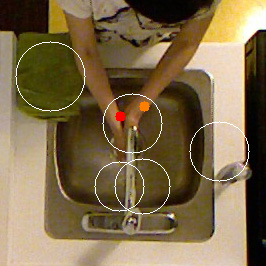
\includegraphics[width=\linewidth]{fig/system/_fast2-rinse1_.jpg} &
%column-3
RINSE
\vskip 0.2cm
$\begin{bmatrix}
0 \\
1.49 \\
-0.16
\end{bmatrix}$ &
%column-4
\begin{minipage}[c]{\linewidth} \centering
[0.27, 0.73, 0.00, 0.00, 0.00, 0.00, 0.00, 0.00] most likely planstep=1
\end{minipage} &
%column-5
$\begin{bmatrix}
2.67 \\
1.21 \\
-0.72
\end{bmatrix}$ &
%column-6
``"use some soap''
\vskip 0.2cm
$\begin{bmatrix}
1.51 \\
0.12 \\
0.52
\end{bmatrix}$ &
%column-7
\vskip 0.15cm
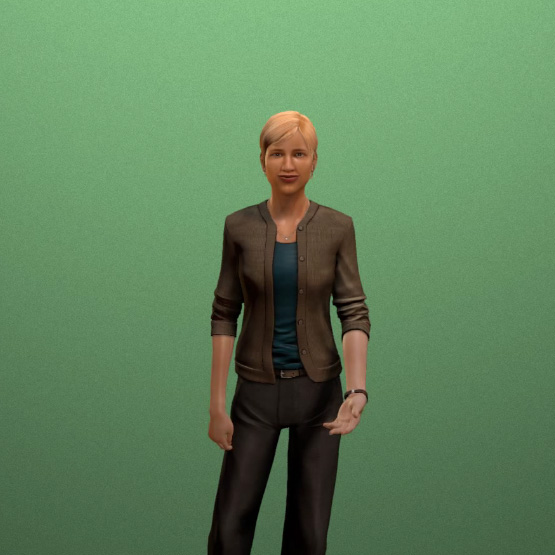
\includegraphics[width=2.6cm]{fig/prompt/_please-use-the-soap_.jpg}
\footnotesize
``You are washing your hands. Please use the soap.''
\\ \hline


%column-1
t4 &
%column-2
\vskip 0.15cm
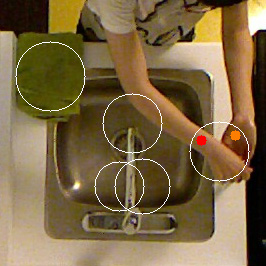
\includegraphics[width=\linewidth]{fig/system/_fast2-soap_.jpg} &
%column-3
SOAP
\vskip 0.2cm
$\begin{bmatrix}
0 \\
0.73 \\
-1.52
\end{bmatrix}$ &
%column-4
\begin{minipage}[c]{\linewidth} \centering
[0.00, 0.01, 0.35, 0.64, 0.00, 0.00, 0.00, 0.00] most likely planstep = 3
\end{minipage} &
%column-5
$\begin{bmatrix}
2.57 \\
0.69 \\
-0.66
\end{bmatrix}$ &
%column-6
N/A &
%column-7
No Prompt
\\ \hline


%column-1
t5 &
%column-2
\vskip 0.15cm
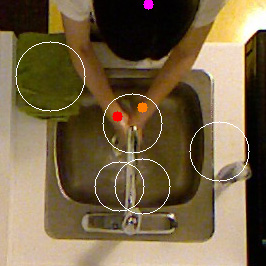
\includegraphics[width=\linewidth]{fig/system/_fast2-rinse_.jpg} &
%column-3
RINSE
\vskip 0.2cm
$\begin{bmatrix}
0 \\
0.23 \\
-1.87
\end{bmatrix}$ &
%column-4
\begin{minipage}[c]{\linewidth} \centering
[0.00, 0.00, 0.01, 0.02, 0.97, 0.00, 0.00, 0.00] most likely planstep = 4
\end{minipage} &
%column-5
$\begin{bmatrix}
2.92 \\
0.7 \\
-0.43
\end{bmatrix}$ &
%column-6
N/A &
%column-7
No Prompt
\\ \hline


%column-1
t6 &
%column-2
\vskip 0.15cm
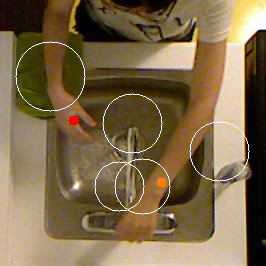
\includegraphics[width=\linewidth]{fig/system/_fast2-tap2_.jpg} &
%column-3
TAP
\vskip 0.2cm
$\begin{bmatrix}
0 \\
1.79 \\
-1.84
\end{bmatrix}$ &
%column-4
\begin{minipage}[c]{\linewidth} \centering
[0.00, 0.00, 0.00, 0.00, 0.18, 0.00, 0.82, 0.00] most likely planstep = 6
\end{minipage} &
%column-5
$\begin{bmatrix}
3.21 \\
0.98 \\
-0.47
\end{bmatrix}$ &
%column-6
N/A &
%column-7
No Prompt
\\ \hline


%column-1
t7 &
%column-2
\vskip 0.15cm
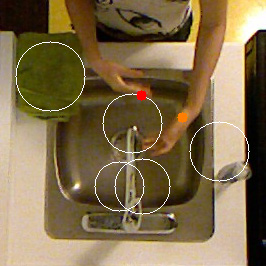
\includegraphics[width=\linewidth]{fig/system/_fast2-rinse3_.jpg} &
%column-3
RINSE
\vskip 0.2cm
$\begin{bmatrix}
0 \\
1.69 \\
-1.6
\end{bmatrix}$ &
%column-4
\begin{minipage}[c]{\linewidth} \centering
[0.00, 0.00, 0.00, 0.00, 0.21, 0.00, 0.79, 0.00] most likely planstep = 6
\end{minipage} &
%column-5
$\begin{bmatrix}
3.27 \\
1.07 \\
-0.58
\end{bmatrix}$ &
%column-6
``use towel''
\vskip 0.2cm
$\begin{bmatrix}
1.77 \\
0.16 \\
1
\end{bmatrix}$ &
%column-7
\vskip 0.15cm
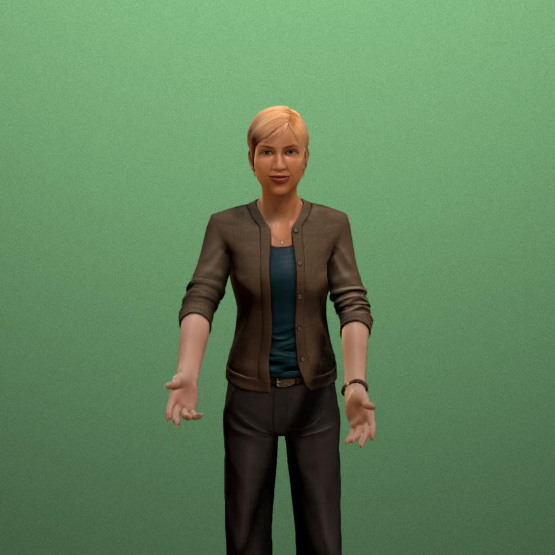
\includegraphics[width=2.6cm]{fig/prompt/_can-i-get-your-hands-dried-up_.jpg}
\footnotesize
``Can I get your hands dried up?''
\\ \hline


%column-1
t8 &
%column-2
\vskip 0.15cm
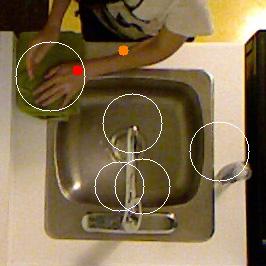
\includegraphics[width=\linewidth]{fig/system/_fast2-towel2_.jpg} &
%column-3
TOWEL
\vskip 0.2cm
$\begin{bmatrix}
0 \\
1.08 \\
-1.16
\end{bmatrix}$ &
%column-4
\begin{minipage}[c]{\linewidth} \centering
[0.00, 0.00, 0.00, 0.00, 0.00, 0.14, 0.00, 0.86] most likely planstep = 7
\end{minipage} &
%column-5
$\begin{bmatrix}
3.31 \\
1.04 \\
-0.57
\end{bmatrix}$ &
%column-6
``all done''
\vskip 0.2cm
$\begin{bmatrix}
1.55 \\
0.38 \\
0.87
\end{bmatrix}$ &
%column-7
\vskip 0.15cm
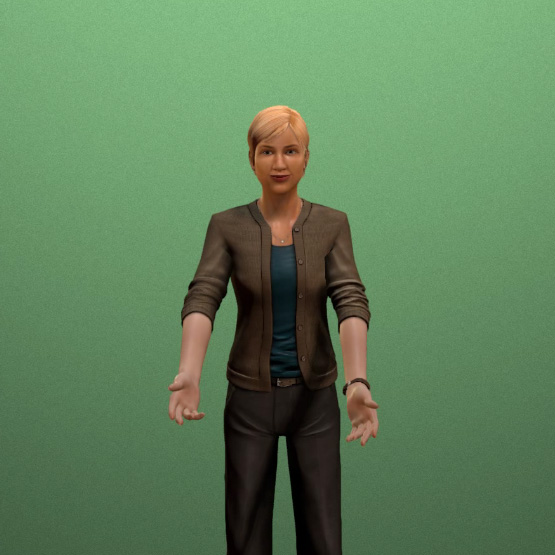
\includegraphics[width=2.6cm]{fig/prompt/_can-you-come-back-soon_.jpg}
\footnotesize
``Can you come back soon?''
\\ \hline

\end{longtable}
\end{center}



%
% Table: results of test #2

\begin{table}
\centering
\caption{State changes in test \#2 of the system}
\label{table:result-2}
\begin{tabular}{| V{0.8cm} | V{2.6cm} | V{1.7cm} | V{2.1cm} | V{1.45cm} | V{1.6cm} | V{3.2cm} |}
\hline

Time &
User Behav. (screenshot) &
Behav. prop./epa &
Planstep Belief &
$f\_c$ &
Prompt: prop./epa &
Avatar (screenshot) \\ \hline


%column-1
t1 &
%column-2
\vskip 0.15cm
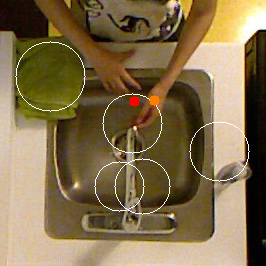
\includegraphics[width=\linewidth]{fig/system/_slow2-rinse1_.jpg} &
%column-3
RINSE
\vskip 0.2cm
$\begin{bmatrix}
0 \\
0.29 \\
-1.86
\end{bmatrix}$ &
%column-4
\begin{minipage}[c]{\linewidth} \centering
[1.00, 0.00, 0.00, 0.00, 0.00, 0.00, 0.00, 0.00] most likely planstep = 0
\end{minipage} &
%column-5
$\begin{bmatrix}
-0.87 \\
-0.28 \\
-2.11
\end{bmatrix}$ &
%column-6
``turn on water''
\vskip 0.2cm
$\begin{bmatrix}
0.87 \\
0.85 \\
0.27
\end{bmatrix}$ &
%column-7
\vskip 0.15cm
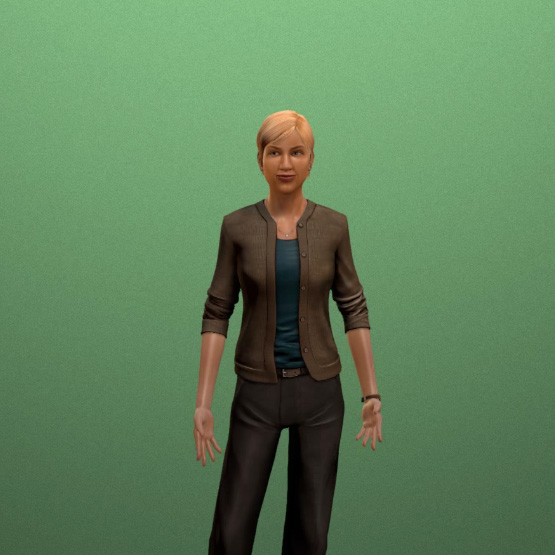
\includegraphics[width=2.6cm]{fig/prompt/_i-want-you-to-turn-the-water-on_.jpg}
\footnotesize
``I want you to turn the water on.''
\\ \hline


%column-1
t2 &
%column-2
\vskip 0.15cm
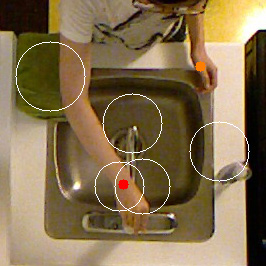
\includegraphics[width=\linewidth]{fig/system/_fast2-tap1_.jpg} &
%column-3
TAP
\vskip 0.2cm
$\begin{bmatrix}
0 \\
1.68 \\
-0.58
\end{bmatrix}$ &
%column-4
\begin{minipage}[c]{\linewidth} \centering
[0.26, 0.74, 0.00, 0.00, 0.00, 0.00, 0.00, 0.00] most likely planstep=1
\end{minipage} &
%column-5
$\begin{bmatrix}
2.73 \\
1.14 \\
-1.03
\end{bmatrix}$ &
%column-6
N/A &
%column-7
No Prompt
\\ \hline


%column-1
t3 &
%column-2
\vskip 0.15cm
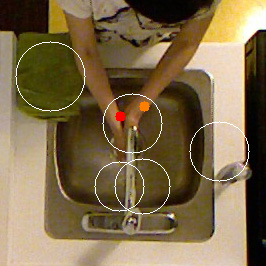
\includegraphics[width=\linewidth]{fig/system/_fast2-rinse1_.jpg} &
%column-3
RINSE
\vskip 0.2cm
$\begin{bmatrix}
0 \\
1.49 \\
-0.16
\end{bmatrix}$ &
%column-4
\begin{minipage}[c]{\linewidth} \centering
[0.27, 0.73, 0.00, 0.00, 0.00, 0.00, 0.00, 0.00] most likely planstep=1
\end{minipage} &
%column-5
$\begin{bmatrix}
2.67 \\
1.21 \\
-0.72
\end{bmatrix}$ &
%column-6
``"use some soap''
\vskip 0.2cm
$\begin{bmatrix}
1.51 \\
0.12 \\
0.52
\end{bmatrix}$ &
%column-7
\vskip 0.15cm
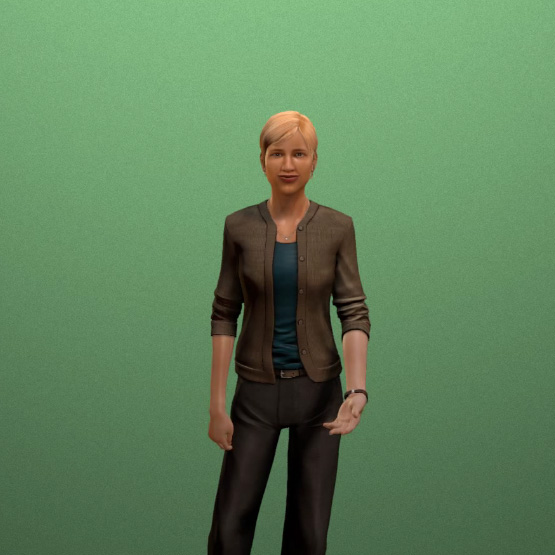
\includegraphics[width=2.6cm]{fig/prompt/_please-use-the-soap_.jpg}
\footnotesize
``You are washing your hands. Please use the soap.''
\\ \hline


%column-1
t4 &
%column-2
\vskip 0.15cm
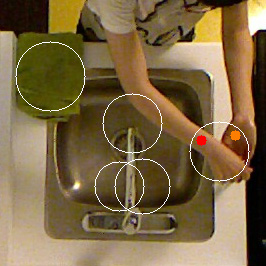
\includegraphics[width=\linewidth]{fig/system/_fast2-soap_.jpg} &
%column-3
SOAP
\vskip 0.2cm
$\begin{bmatrix}
0 \\
0.73 \\
-1.52
\end{bmatrix}$ &
%column-4
\begin{minipage}[c]{\linewidth} \centering
[0.00, 0.01, 0.35, 0.64, 0.00, 0.00, 0.00, 0.00] most likely planstep = 3
\end{minipage} &
%column-5
$\begin{bmatrix}
2.57 \\
0.69 \\
-0.66
\end{bmatrix}$ &
%column-6
N/A &
%column-7
No Prompt
\\ \hline


%column-1
t5 &
%column-2
\vskip 0.15cm
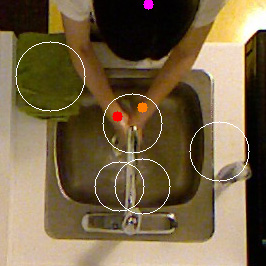
\includegraphics[width=\linewidth]{fig/system/_fast2-rinse_.jpg} &
%column-3
RINSE
\vskip 0.2cm
$\begin{bmatrix}
0 \\
0.23 \\
-1.87
\end{bmatrix}$ &
%column-4
\begin{minipage}[c]{\linewidth} \centering
[0.00, 0.00, 0.01, 0.02, 0.97, 0.00, 0.00, 0.00] most likely planstep = 4
\end{minipage} &
%column-5
$\begin{bmatrix}
2.92 \\
0.7 \\
-0.43
\end{bmatrix}$ &
%column-6
N/A &
%column-7
No Prompt
\\ \hline


%column-1
t6 &
%column-2
\vskip 0.15cm
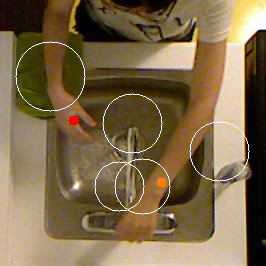
\includegraphics[width=\linewidth]{fig/system/_fast2-tap2_.jpg} &
%column-3
TAP
\vskip 0.2cm
$\begin{bmatrix}
0 \\
1.79 \\
-1.84
\end{bmatrix}$ &
%column-4
\begin{minipage}[c]{\linewidth} \centering
[0.00, 0.00, 0.00, 0.00, 0.18, 0.00, 0.82, 0.00] most likely planstep = 6
\end{minipage} &
%column-5
$\begin{bmatrix}
3.21 \\
0.98 \\
-0.47
\end{bmatrix}$ &
%column-6
N/A &
%column-7
No Prompt
\\ \hline


%column-1
t7 &
%column-2
\vskip 0.15cm
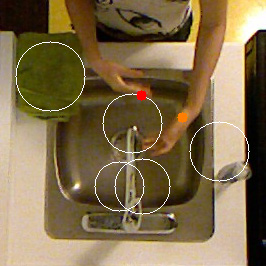
\includegraphics[width=\linewidth]{fig/system/_fast2-rinse3_.jpg} &
%column-3
RINSE
\vskip 0.2cm
$\begin{bmatrix}
0 \\
1.69 \\
-1.6
\end{bmatrix}$ &
%column-4
\begin{minipage}[c]{\linewidth} \centering
[0.00, 0.00, 0.00, 0.00, 0.21, 0.00, 0.79, 0.00] most likely planstep = 6
\end{minipage} &
%column-5
$\begin{bmatrix}
3.27 \\
1.07 \\
-0.58
\end{bmatrix}$ &
%column-6
``use towel''
\vskip 0.2cm
$\begin{bmatrix}
1.77 \\
0.16 \\
1
\end{bmatrix}$ &
%column-7
\vskip 0.15cm
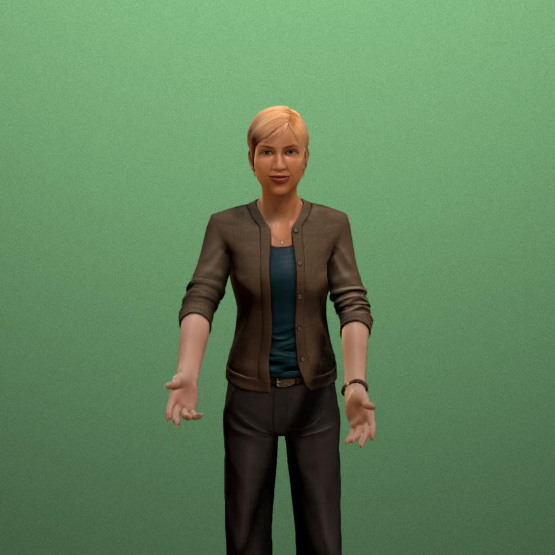
\includegraphics[width=2.6cm]{fig/prompt/_can-i-get-your-hands-dried-up_.jpg}
\footnotesize
``Can I get your hands dried up?''
\\ \hline


%column-1
t8 &
%column-2
\vskip 0.15cm
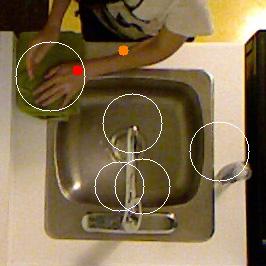
\includegraphics[width=\linewidth]{fig/system/_fast2-towel2_.jpg} &
%column-3
TOWEL
\vskip 0.2cm
$\begin{bmatrix}
0 \\
1.08 \\
-1.16
\end{bmatrix}$ &
%column-4
\begin{minipage}[c]{\linewidth} \centering
[0.00, 0.00, 0.00, 0.00, 0.00, 0.14, 0.00, 0.86] most likely planstep = 7
\end{minipage} &
%column-5
$\begin{bmatrix}
3.31 \\
1.04 \\
-0.57
\end{bmatrix}$ &
%column-6
``all done''
\vskip 0.2cm
$\begin{bmatrix}
1.55 \\
0.38 \\
0.87
\end{bmatrix}$ &
%column-7
\vskip 0.15cm
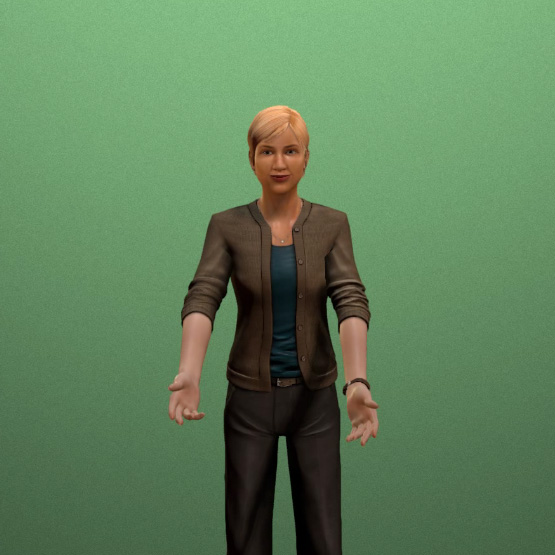
\includegraphics[width=2.6cm]{fig/prompt/_can-you-come-back-soon_.jpg}
\footnotesize
``Can you come back soon?''
\\ \hline

\end{tabular}
\end{table}


